%% This is a tikz file
%% This template was modified from 'gecko-tree-3.tikz.tex' output by ../bin/plot-tree.py

\tikzset{node lower left/.style={font=\small,anchor=north east,text height=0.240cm,text depth=0.068cm,inner sep=0.03cm},
leaf/.style={font=\small,anchor=west,text height=0.240cm,text depth=0.068cm},
node upper left/.style={font=\small,anchor=south east,text height=0.240cm,text depth=0.068cm,inner sep=0.03cm},
bracket label/.style={font=\small,anchor=west,text height=0.240cm,text depth=0.068cm,inner sep=0.1cm},
node upper right/.style={font=\small,anchor=south west,text height=0.240cm,text depth=0.068cm,inner sep=0.03cm},
node right/.style={font=\small,anchor=west,text height=0.240cm,text depth=0.068cm,inner sep=0.03cm},
branch/.style={font=\tiny,text height=0.144cm,text depth=0.041cm,inner sep=0.025cm},
root/.style={font=\small,anchor=east,text height=0.240cm,text depth=0.068cm},
node lower right/.style={font=\small,anchor=north west,text height=0.240cm,text depth=0.068cm,inner sep=0.03cm}}

% \begin{tikzpicture}[ultra thick,inner sep=0.1cm]
\begin{tikzpicture}[line width=3pt,inner sep=0.1cm]
%  3:\hspace{15mm}\includegraphics[width=12mm,resolution=150]{../images/gekko-vittatus-1-red-shadow.png}
% +2:$T_1$
% |4:\hspace{15mm}\includegraphics[width=12mm,resolution=150]{../images/gekko-vittatus-2-orange-shadow.png}
% |
% 07:\hspace{15mm}\includegraphics[width=12mm,resolution=150]{../images/gekko-vittatus-3-yellow-shadow.png}
% 6:$T_2$
% |8:\hspace{15mm}\includegraphics[width=12mm,resolution=150]{../images/gekko-vittatus-4-green-shadow.png}
% 5
% |10:\hspace{15mm}\includegraphics[width=12mm,resolution=150]{../images/gekko-vittatus-5-blue-shadow.png}
% +9:$T_3$
%  11:\hspace{15mm}\includegraphics[width=12mm,resolution=150]{../images/gekko-vittatus-6-violet-shadow.png}

% The scale is 1.000000, and the yScale is 1.000000

%% Coordinates of nodes.
\coordinate (n0) at (0.000,3.000);
\coordinate (n1) at (0.100,3.000);
\coordinate (n1p) at (0.000,3.000);
\coordinate (n2) at (\firstdepth,4.500);
\coordinate (n2p) at (0.100,4.500);
\coordinate (n3) at (5.600,5.000);
\coordinate (n3p) at (\firstdepth,5.000);
\coordinate (n4) at (5.600,4.000);
\coordinate (n4p) at (\firstdepth,4.000);
\coordinate (n5) at (0.600,1.500);
\coordinate (n5p) at (0.100,1.500);
\coordinate (n6) at (\seconddepth,2.500);
\coordinate (n6p) at (0.600,2.500);
\coordinate (n7) at (5.600,3.000);
\coordinate (n7p) at (\seconddepth,3.000);
\coordinate (n8) at (5.600,2.000);
\coordinate (n8p) at (\seconddepth,2.000);
\coordinate (n9) at (\thirddepth,0.500);
\coordinate (n9p) at (0.600,0.500);
\coordinate (n10) at (5.600,1.000);
\coordinate (n10p) at (\thirddepth,1.000);
\coordinate (n11) at (5.600,0.000);
\coordinate (n11p) at (\thirddepth,0.000);


%% maintain canvas size for pair plot
\maintainTreeCanvasSize{\draw [black!00] (n1p) -- (n1);}
\maintainTreeCanvasSize{\draw [black!00] (n2p) -- (n2);}
\maintainTreeCanvasSize{\draw [black!00] (n5p) -- (n5);}
\maintainTreeCanvasSize{\draw [black!00] (n6p) -- (n6);}
\maintainTreeCanvasSize{\draw [black!00] (n9p) -- (n9);}
\maintainTreeCanvasSize{\draw [black!00, line cap=rect] (n2p) -- (n5p);}
\maintainTreeCanvasSize{\draw [black!00, line cap=rect] (n6p) -- (n9p);}

%% events
\draw [\firstEventLineColor,dashed] (\firstdepth,-0.500) -- (\firstdepth,5.500);
\includeEventLabels{\node [text=\firstEventLabelColor,font=\LARGE,yshift=0.300cm,text height=0.415cm,text depth=0.118cm] at (\firstdepth,5.500) {\getEventLabel{\firstdepth}};}

\ifthenelse{\equal{\firstdepth}{\seconddepth}}{}{
\draw [\secondEventLineColor,dashed] (\seconddepth,-0.500) -- (\seconddepth,5.500);
\includeEventLabels{\node [text=\secondEventLabelColor,font=\LARGE,yshift=0.300cm,text height=0.415cm,text depth=0.118cm] at (\seconddepth,5.500) {\getEventLabel{\seconddepth}};}
}

\ifthenelse{\equal{\firstdepth}{\thirddepth} \OR \equal{\seconddepth}{\thirddepth}}{}{
\draw [\thirdEventLineColor,dashed] (\thirddepth,-0.500) -- (\thirddepth,5.500);
\includeEventLabels{\node [text=\thirdEventLabelColor,font=\LARGE,yshift=0.300cm,text height=0.415cm,text depth=0.118cm] at (\thirddepth,5.500) {\getEventLabel{\thirddepth}};}
}

%% horizontal lines
\ignoreForPairs{\draw (n1p) -- (n1);}
\ignoreForPairs{\draw (n2p) -- (n2);}
\draw (n3p) -- (n3);
\draw (n4p) -- (n4);
\ignoreForPairs{\draw (n5p) -- (n5);}
\ignoreForPairs{\draw (n6p) -- (n6);}
\draw (n7p) -- (n7);
\draw (n8p) -- (n8);
\ignoreForPairs{\draw (n9p) -- (n9);}
\draw (n10p) -- (n10);
\draw (n11p) -- (n11);

%% vertical lines
\ignoreForPairs{\draw [line cap=rect] (n2p) -- (n5p);}
\draw [line cap=rect] (n3p) -- (n4p);
\ignoreForPairs{\draw [line cap=rect] (n6p) -- (n9p);}
\draw [line cap=rect] (n7p) -- (n8p);
\draw [line cap=rect] (n10p) -- (n11p);

%% show pairs only 
\includeForPairs{
    \coordinate (n2m) at (\maximumdepth-\stemlength,4.500);
    \coordinate (n2s) at (\firstdepth-\stemlength,4.500);
    \coordinate (n6s) at (\seconddepth-\stemlength,2.500);
    \coordinate (n9s) at (\thirddepth-\stemlength,0.500);
    \maintainPairCanvasSize{\draw [black!00] (n2m) -- (n2);}
    \draw (n2s) -- (n2);
    \draw (n6s) -- (n6);
    \draw (n9s) -- (n9);
}


%% leaf labels
\node [right=0mm of n3] {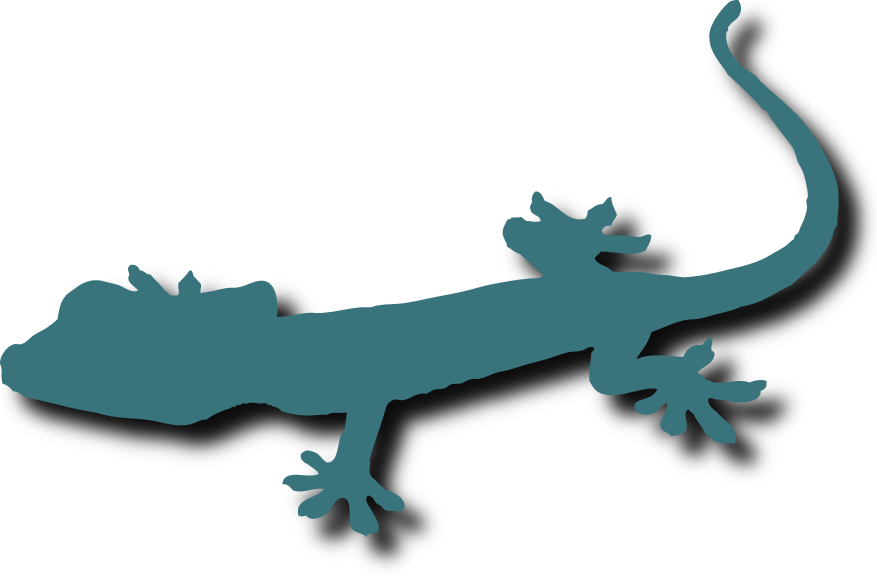
\includegraphics[width=14mm]{../phylopics/gekko-vittatus-5-teal-shadow.png}};
\node [right=0mm of n4] {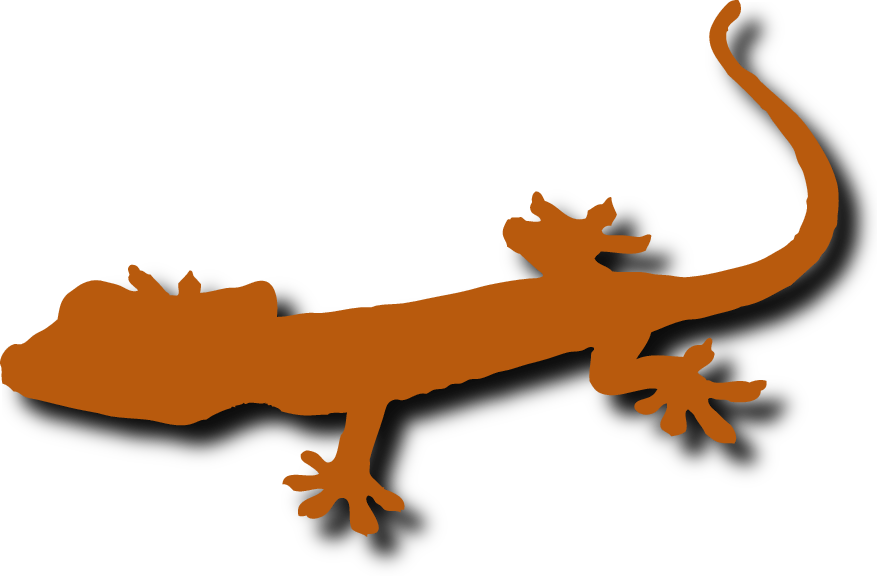
\includegraphics[width=14mm]{../phylopics/gekko-vittatus-6-auburn-shadow.png}};
\node [right=0mm of n7] {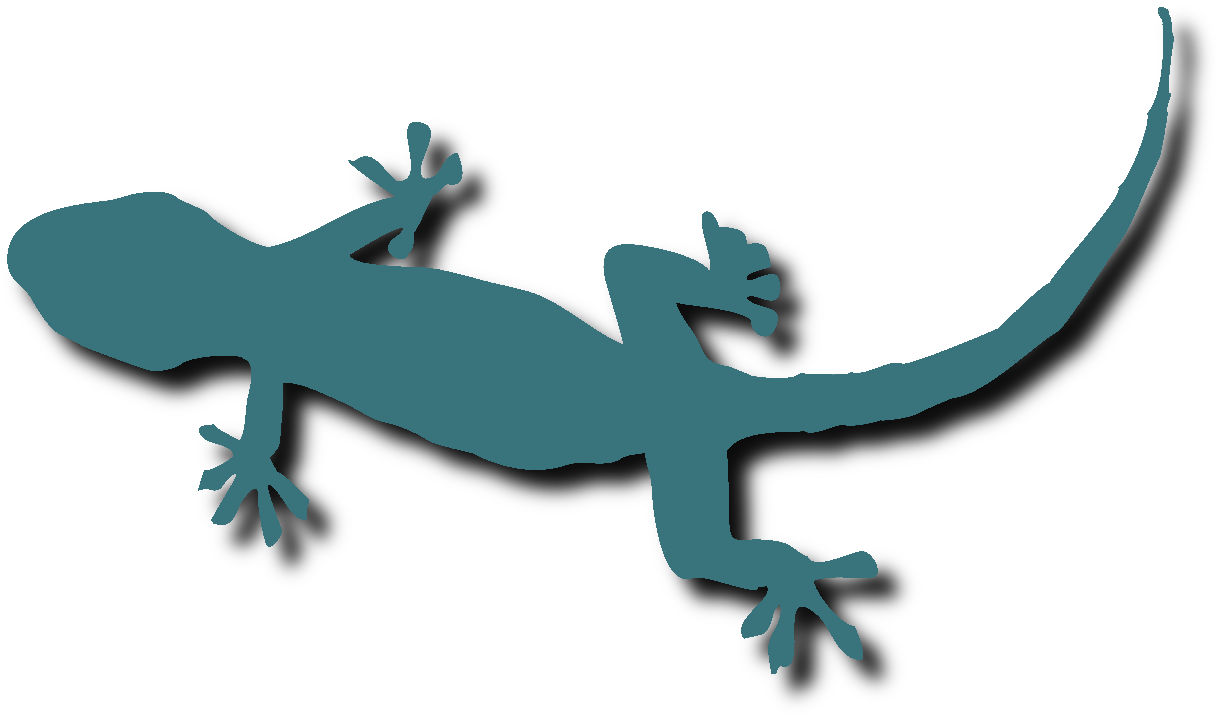
\includegraphics[width=14mm]{../phylopics/gecko-pixabay-cc0-5-teal-shadow.png}};
\node [right=0mm of n8] {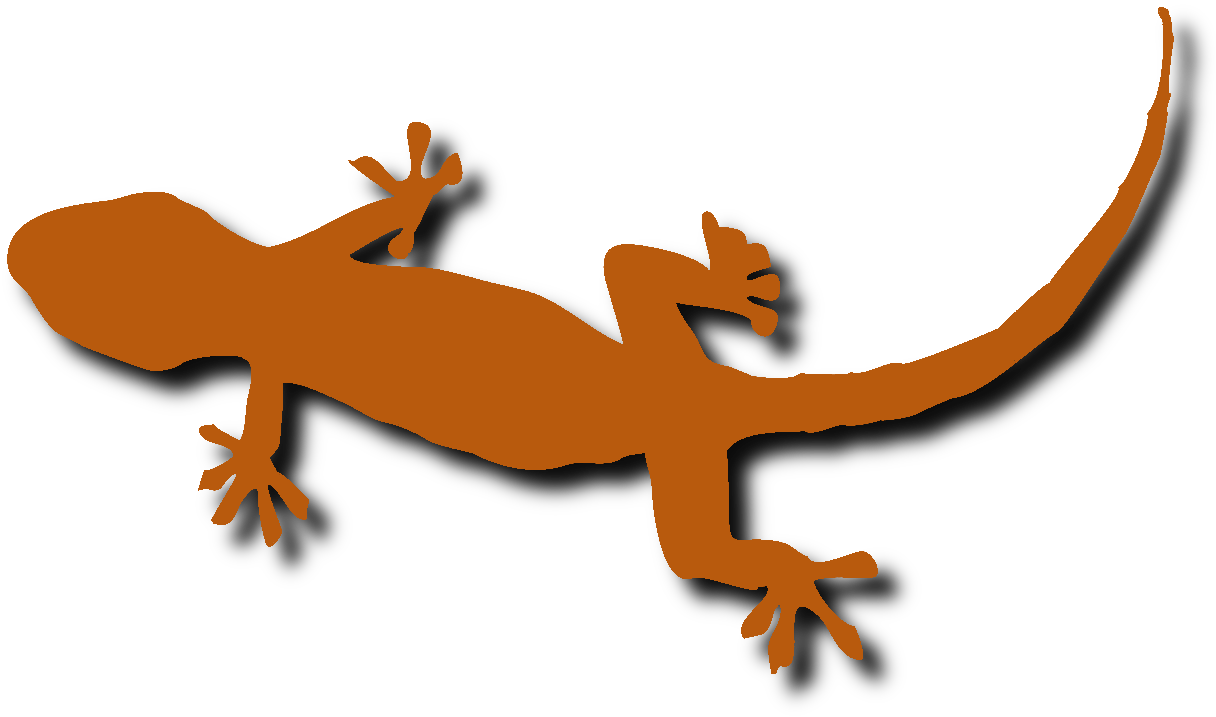
\includegraphics[width=14mm]{../phylopics/gecko-pixabay-cc0-6-auburn-shadow.png}};
\node [right=0mm of n10] {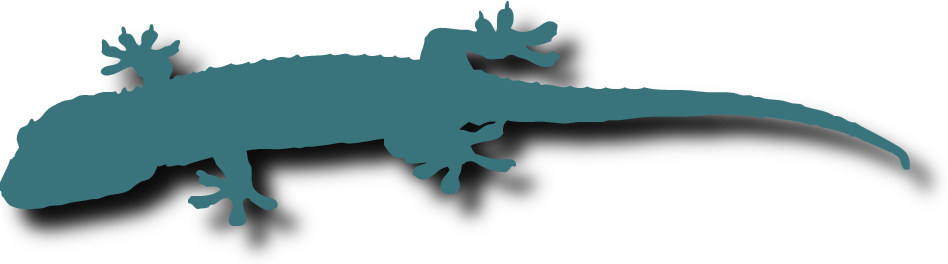
\includegraphics[width=14mm]{../phylopics/gekko-gecko-5-teal-shadow.png}};
\node [right=0mm of n11] {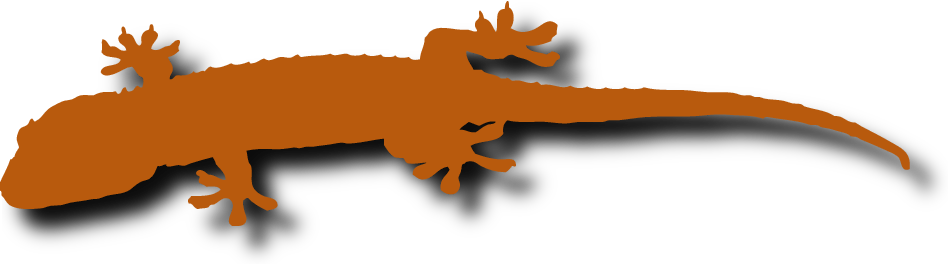
\includegraphics[width=14mm]{../phylopics/gekko-gecko-6-auburn-shadow.png}};

% internal node labels (doSmartLabels is True)
% \includeNodeLabels{\node [node right] at (n2) {$T_1$};}
% \includeNodeLabels{\node [node right] at (n6) {$T_2$};}
% \includeNodeLabels{\node [node right] at (n9) {$T_3$};}

\end{tikzpicture}
